\section{BAO fits}
\label{sec:fits}

\textcolor{red}{one or two options for the model. nuisance parameters.}
\textcolor{red}{Glam template. Linear template.}
\textcolor{red}{spread of measured alpha over 25 FirstGens}
\textcolor{red}{alongside with alpha fits to the power spectrum}
\textcolor{red}{experiment with some choices.}
\textcolor{red}{sigma alpha from the posterior (as a function of k)}
\textcolor{red}{min $\chi^{2}$ vs alpha for P(k), B(k1, k2, k3), P+B BAO and BAOless templates. Look into the scatter in the detection significance across the realizations.}




Below we summarize the mean of the posterior mean estimates, standard deviation, and 4-th and 96-th quantiles from simulations. 

\begin{table}
\caption{‌BAO Constraints from LRG simulations}
\begin{center}
\begin{tabular}{ccccccc}
Stat & Temp & Cov &$< \alpha >$ & $\sigma(\alpha) $ & 4\%&96\%\\
\hline
                            B  &       NASA & full & 0.957 & 0.010& 0.005 & 0.010\\ 
 &       NASA & diagonal & 0.954 & 0.008 &0.003 &0.007\\ 
\hline
                            B  &   fiducial & full & 0.998 & 0.002& 0.001 & 0.002\\ 
 &   fiducial & diagonal & 0.997 & 0.001 &0.001 &0.003\\ 
\hline
                    Reduced B  &       NASA & full & 0.961 & 0.009& 0.005 & 0.012\\ 
 &       NASA & diagonal & 0.958 & 0.009 &0.007 &0.013\\ 
\hline
                    Reduced B  &   fiducial & full & 1.002 & 0.009& 0.004 & 0.008\\ 
 &   fiducial & diagonal & 1.002 & 0.008 &0.008 &0.013\\ 
\hline
                            P  &       NASA & full & 0.959 & 0.005& 0.002 & 0.006\\ 
 &       NASA & diagonal & 0.958 & 0.005 &0.003 &0.006\\ 
\hline
                            P  &   fiducial & full & 1.000 & 0.003& 0.004 & 0.005\\ 
 &   fiducial & diagonal & 1.001 & 0.004 &0.004 &0.00
\end{tabular}
\end{center}
\label{tab:lrg}
\end{table}


\begin{table}
\caption{‌BAO Constraints from ELG simulations}
\begin{center}
\begin{tabular}{ccccccc}
Stat & Temp & Cov &$< \alpha >$ & $\sigma(\alpha) $ & 4\%&96\%\\
\hline
                            B  &       NASA & full & 0.961 & 0.018& 0.007 & 0.014\\ 
 &       NASA & diagonal & 0.953 & 0.010 &0.006 &0.010\\ 
\hline
                            B  &   fiducial & full & 0.998 & 0.001& 0.001 & 0.002\\ 
 &   fiducial & diagonal & 0.997 & 0.001 &0.001 &0.003\\ 
\hline
                    Reduced B  &       NASA & full & 0.960 & 0.014& 0.006 & 0.013\\ 
 &       NASA & diagonal & 0.956 & 0.012 &0.011 &0.016\\ 
\hline
                    Reduced B  &   fiducial & full & 1.002 & 0.011& 0.004 & 0.010\\ 
 &   fiducial & diagonal & 1.003 & 0.010 &0.009 &0.017\\ 
\hline
                            P  &       NASA & full & 0.951 & 0.004& 0.002 & 0.004\\ 
 &       NASA & diagonal & 0.951 & 0.003 &0.003 &0.004\\ 
\hline
                            P  &   fiducial & full & 1.000 & 0.003& 0.003 & 0.004\\ 
 &   fiducial & diagonal & 1.000 & 0.003 &0.003 &0.005
\end{tabular}
\end{center}
\label{label:elg}
\end{table}


\begin{table}
\caption{‌BAO Constraints from QSO simulations}
\begin{center}
\begin{tabular}{ccccccc}
Stat & Temp & Cov &$< \alpha >$ & $\sigma(\alpha) $ & 4\%&96\%\\
\hline
                            B  &       NASA & full & 0.962 & 0.012& 0.006 & 0.012\\ 
 &       NASA & diagonal & 0.961 & 0.012 &0.003 &0.008\\ 
\hline
                            B  &   fiducial & full & 0.997 & 0.002& 0.001 & 0.003\\ 
 &   fiducial & diagonal & 0.996 & 0.002 &0.001 &0.003\\ 
\hline
                    Reduced B  &       NASA & full & 0.965 & 0.012& 0.004 & 0.015\\ 
 &       NASA & diagonal & 0.962 & 0.012 &0.007 &0.018\\ 
\hline
                    Reduced B  &   fiducial & full & 1.003 & 0.017& 0.007 & 0.014\\ 
 &   fiducial & diagonal & 1.000 & 0.014 &0.013 &0.021\\ 
\hline
                            P  &       NASA & full & 0.963 & 0.008& 0.002 & 0.006\\ 
 &       NASA & diagonal & 0.961 & 0.008 &0.003 &0.008\\ 
\hline
                            P  &   fiducial & full & 1.001 & 0.008& 0.006 & 0.009\\ 
 &   fiducial & diagonal & 1.001 & 0.008 &0.007 &0.011
\end{tabular}
\end{center}
\label{label:qso}
\end{table}




% \begin{figure*}
% 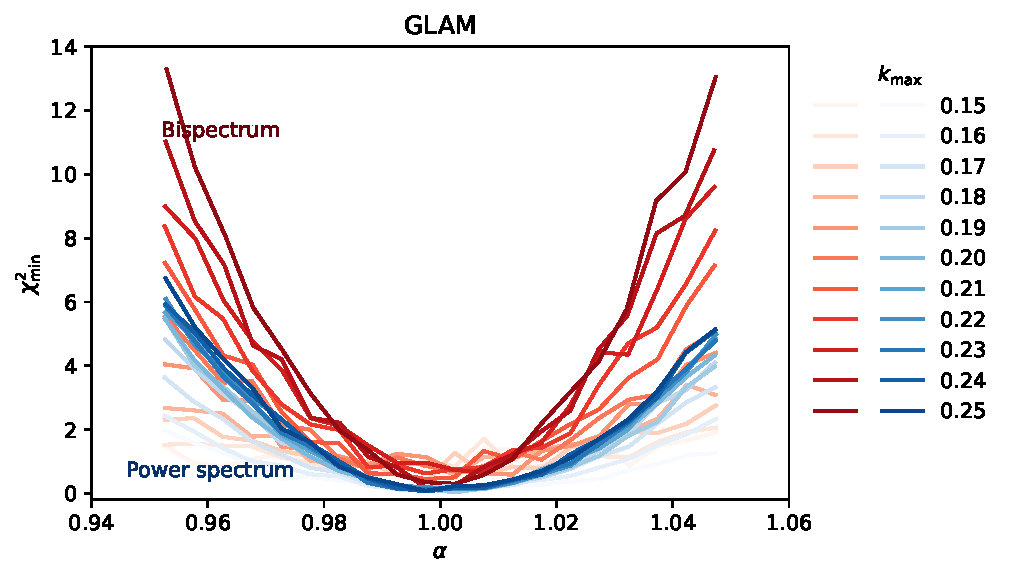
\includegraphics[width=0.48\textwidth]{chi2_GLAM.pdf}
% 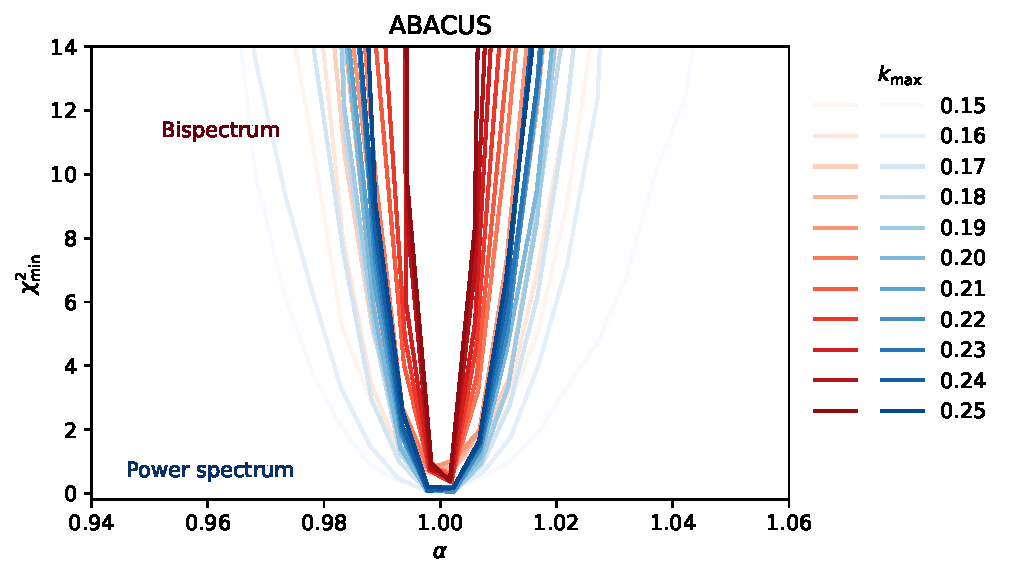
\includegraphics[width=0.48\textwidth]{chi2_ABACUS.pdf}
% 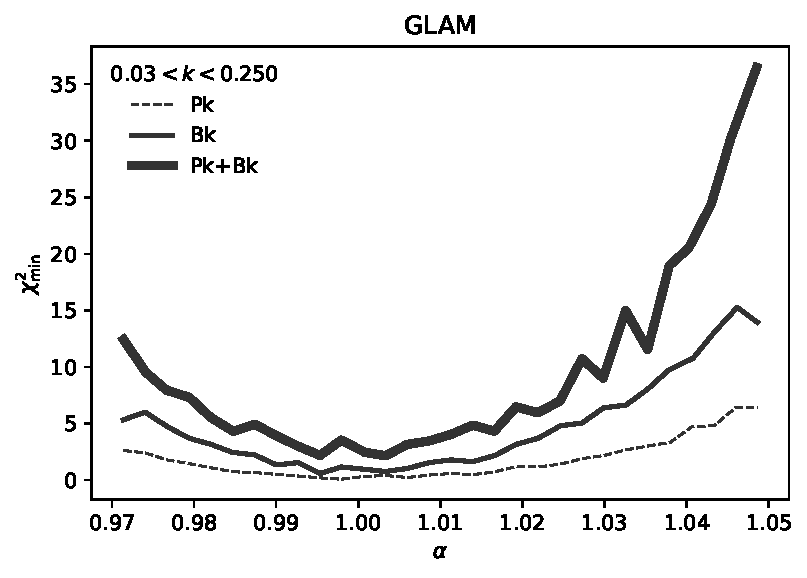
\includegraphics[width=0.48\textwidth]{chi2alpha_glam.pdf}
% 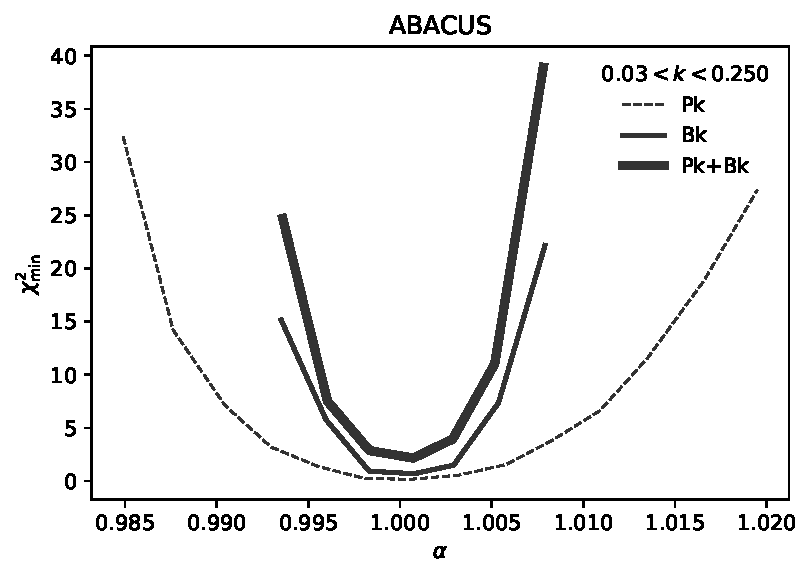
\includegraphics[width=0.48\textwidth]{chi2alpha_abacus.pdf}
% \caption{Marginalized minimum $\chi^{2}$ as a function of the BAO peak $\alpha$}\label{fig:chi2alpha}
% \end{figure*}

% \begin{figure*}
% 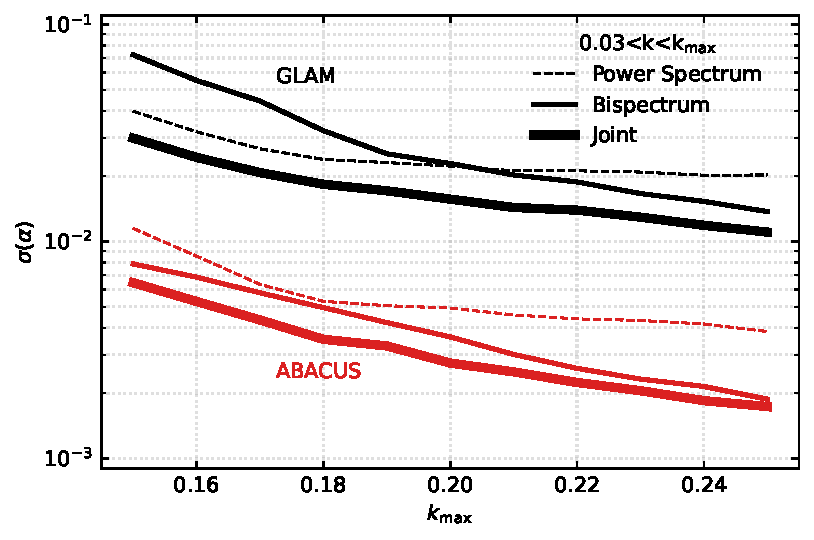
\includegraphics[width=0.9\textwidth]{sigma_kmax.pdf}
% \caption{Dispersion in the BAO peak $\alpha$ as a function of the maximum wavenumber $k_{\rm max}$}
% \end{figure*}